\documentclass[12pt, a4paper]{article}
\usepackage[utf8]{inputenc}
\usepackage[T1]{fontenc}
\usepackage[brazil]{babel}
\usepackage{amsmath, amsfonts, amssymb}
\usepackage{graphicx}
\usepackage{geometry}
\usepackage{setspace}
\usepackage{indentfirst}
\usepackage{caption}
\usepackage{subcaption}
\usepackage{cite}
\usepackage{listings}
\usepackage{xcolor}
\usepackage{booktabs}
\usepackage{array}
\usepackage{multirow}
\usepackage{algorithm}
\usepackage{algpseudocode}
\usepackage{fancyhdr}
\usepackage{hyperref}
\usepackage{siunitx}
\usepackage{mathtools}
\usepackage{float}
\usepackage{enumitem}
\usepackage{mdframed}
\usepackage{tcolorbox}
\tcbuselibrary{skins,breakable}

\geometry{left=3cm, top=3cm, right=2cm, bottom=2cm}
\onehalfspacing

% ─── Cores ────────────────────────────────────────────────────────────────────
\definecolor{codegray}{rgb}{0.96,0.96,0.96}
\definecolor{codeblue}{rgb}{0.0,0.0,0.6}
\definecolor{codegreen}{rgb}{0.0,0.45,0.0}
\definecolor{codepurple}{rgb}{0.5,0.0,0.6}
\definecolor{codered}{rgb}{0.6,0.0,0.0}
\definecolor{aquacolor}{rgb}{0.0,0.50,0.55}
\definecolor{boxblue}{rgb}{0.88,0.93,0.98}
\definecolor{boxgreen}{rgb}{0.88,0.97,0.88}

% ─── Listagens de código ──────────────────────────────────────────────────────
\lstset{
  basicstyle=\ttfamily\footnotesize,
  backgroundcolor=\color{codegray},
  frame=single, rulecolor=\color{gray!50},
  breaklines=true,
  keywordstyle=\color{codeblue}\bfseries,
  commentstyle=\color{codegreen}\itshape,
  stringstyle=\color{codepurple},
  numbers=left, numberstyle=\tiny\color{gray}, numbersep=6pt,
  tabsize=2, showspaces=false, showstringspaces=false,
  captionpos=b,
}
\lstdefinelanguage{ArduinoC}[]{C}{
  morekeywords={analogRead,digitalWrite,Serial,delay,pinMode,INPUT,OUTPUT,HIGH,LOW,
                String,bool,float,int,void,const,return,true,false},
}

% ─── Caixas de destaque ───────────────────────────────────────────────────────
\newtcolorbox{conceitobox}[1][]{
  colback=boxblue, colframe=aquacolor!80!black,
  fonttitle=\bfseries, title=#1, breakable, before upper=\setlength{\parskip}{4pt}
}
\newtcolorbox{resultadobox}[1][]{
  colback=boxgreen, colframe=codegreen!70!black,
  fonttitle=\bfseries, title=#1, breakable
}

% ─── Cabeçalho ────────────────────────────────────────────────────────────────
\pagestyle{fancy}\fancyhf{}
\rhead{\footnotesize Aqua Monitor -- Relatorio Tecnico Final -- UFAM/FT 2026}
\lhead{\footnotesize Engenharia da Computacao | Microeletronica}
\rfoot{\thepage}

\hypersetup{colorlinks=true, linkcolor=aquacolor!80!black, citecolor=codeblue, urlcolor=codeblue}

\begin{document}

%% ──────────────────────────────────────────────────────────────────────────────
%%  CAPA
%% ──────────────────────────────────────────────────────────────────────────────
\begin{titlepage}
\begin{center}
  {\Large\bfseries Universidade Federal do Amazonas -- UFAM}\\[0.2cm]
  {\large\bfseries Faculdade de Tecnologia -- FT}\\[0.1cm]
  {\large\bfseries Curso de Engenharia da Computacao}\\[1.8cm]

  {\large\bfseries Matheus Serrao Uchoa \quad Matricula: 22052633}\\[0.3cm]
  {\large\bfseries [Nome Componente 2] \quad Matricula: [Inserir]}\\[1.8cm]

  {\LARGE\bfseries RELATORIO TECNICO FINAL\\[0.3cm]
   Unidade 7 $|$ Capitulo 5 -- Desafio de Design de Circuitos Integrados}\\[0.7cm]

  {\Large\bfseries Aqua Monitor: Plataforma IoT de Monitoramento da\\
   Qualidade da Agua em Viveiros de Piscicultura\\[0.4cm]
   com Projeto de Conversor Analogico-Digital\\
   SAR de 4-Bits em Tecnologia CMOS 180nm}\\[1.4cm]

  \vfill
  {\normalsize\textbf{Disciplina:} Design de Circuitos Integrados -- CI Amazonia}\\[0.1cm]
  {\normalsize\textbf{Professor:} Joao Fonseca}\\[0.3cm]
  {\normalsize Manaus -- AM \quad Maio de 2026}
\end{center}
\end{titlepage}

\setcounter{page}{1}
\tableofcontents
\newpage

%% ──────────────────────────────────────────────────────────────────────────────
%%  RESUMO
%% ──────────────────────────────────────────────────────────────────────────────
\begin{abstract}
\noindent
Este relatorio tecnico descreve o desenvolvimento integral do sistema \textbf{Aqua Monitor},
uma plataforma de codigo aberto voltada ao monitoramento continuo da qualidade da agua em
viveiros de piscicultura da regiao amazonica. O sistema e composto por quatro camadas funcionais
integradas: (i)~\textbf{Hardware embarcado} -- microcontrolador ESP32 conectado a quatro sensores
(temperatura DS18B20, pH PH4502C, turbidez SEN0189 e solidos dissolvidos Gravity TDS), com
comunicacao via protocolo MQTT e envio de dados a plataforma de nuvem Firebase/Firestore; (ii)~\textbf{Backend inteligente}
-- servidor Python/FastAPI com agente de linguagem (Ollama qwen2:0.5b) para interpretacao de
perguntas em linguagem natural sobre qualidade da agua; (iii)~\textbf{Aplicativo mobile}
-- desenvolvido em Ionic/React/TypeScript, com monitoramento em tempo real, historico de dados
com graficos, exportacao em PDF e controle remoto do ESP32; (iv)~\textbf{Modulo de microeletronica}
-- projeto de um Conversor Analogico-Digital de Aproximacoes Sucessivas (SAR ADC) de 4~bits em
tecnologia CMOS de $1{,}8\,\text{V}$ (180nm), concebido para substituir o ADC interno do ESP32,
cuja qualidade e degradada pelo ruido radiado pelo modulo Wi-Fi integrado. O projeto do SAR ADC
cobre o fluxo completo de design de circuitos integrados de sinal misto: especificacao eletrica,
Maquina de Estados em Verilog RTL, DAC de redistribuicao de carga ($C_0 = 100\,\text{fF}$,
ruido $kT/C = 1{,}6\,\text{mV}$ com margem de $35\times$ sobre $V_{LSB}/2$), comparador diferencial
PMOS de dois estagios ($A_1 = 95\,\text{V/V}$, $t_{pd} = 7{,}4\,\text{ns}$ pre-layout),
layout fisico Common-Centroid ($4025\,\mu\text{m}^2$), extracao de parasitas e simulacao
pos-layout ($\Delta t_{pd} = +2{,}6\,\text{ns}$, $\Delta V_{th} = 0{,}3\,\text{mV}$),
alem de verificacao LVS sem erros (7 transistores, 10 nos, 0 violacoes). A figura de merito
energetica calculada e $\text{FOM}_{Walden} = 45\,\text{fJ/conv-step}$.\\[0.5em]
\textbf{Palavras-chave:} IoT, Aquicultura, Monitoramento Ambiental, SAR ADC, CMOS 180nm,
Mixed-Signal, Redistribuicao de Carga, Comparador Diferencial, Common-Centroid, Verilog, LVS.
\end{abstract}
\newpage

%% ──────────────────────────────────────────────────────────────────────────────
%%  1. INTRODUCAO
%% ──────────────────────────────────────────────────────────────────────────────
\section{Introducao}

\subsection{Contexto e Motivacao}

A piscicultura e uma das atividades economicas de maior crescimento na regiao Norte do Brasil,
com o Amazonas figurando entre os principais estados produtores. A qualidade da agua e o
fator critico de sucesso: variacoes de pH, temperatura, turbidez ou condutividade fora das
faixas ideais causam estresse nos animais, reducao da imunidade e, em casos extremos, morte
em massa de planteis, com prejuizos que podem chegar a dezenas de milhares de reais por ciclo.
O monitoramento tradicional baseia-se em coletas manuais realizadas uma ou duas vezes ao dia,
o que e insuficiente para detectar eventos rapidos como um pico de amonia ou uma queda brusca
de oxigenio dissolvido~\cite{aquaculture2019}.

O \textbf{Aqua Monitor} nasce para resolver esse problema: uma plataforma de monitoramento
continuo, de baixo custo, conectada a nuvem e acessivel via aplicativo movel, que permite ao
piscicultor acompanhar os parametros da agua de qualquer lugar, a qualquer hora, e receber
alertas imediatos quando valores saem das faixas recomendadas.

\subsection{O Problema da Qualidade de Aquisicao Analogica no ESP32}

O microcontrolador ESP32 -- escolhido pelo custo acessivel e pelo modulo Wi-Fi integrado --
possui internamente um SAR ADC de 12~bits. Contudo, a Espressif, fabricante do chip, documenta
em seu manual tecnico~\cite{espressif2023} que o modulo de radio Wi-Fi 802.11n introduz
\textbf{ruido de modo comum de ate $60\,\text{mV}$} no rail de alimentacao analogica ($AV_{DD}$),
degradando a qualidade das leituras. Para o sensor de pH -- cuja curva de calibracao tem
sensibilidade de apenas $\sim 58\,\text{mV}/\text{pH}$ -- um ruido de $60\,\text{mV}$ representa
mais de $1\,\text{pH}$ de incerteza, tornando as leituras inuteis sem filtragem intensiva.

Esta limitacao justifica o projeto de um \textbf{ADC customizado dedicado}, projetado especificamente
para a faixa dinamica dos sensores do Aqua Monitor, sem a interferencia do transceptor de radio.

\subsection{Escopo e Organizacao deste Relatorio}

Este relatorio apresenta o Aqua Monitor como um produto completo, descrevendo todas as camadas
do sistema com nivel de detalhe suficiente para que qualquer leitor -- independente de
background tecnico -- compreenda o que foi construido, por que cada decisao de design foi
tomada, e o que cada componente faz. A organizacao e a seguinte:

\begin{itemize}
  \item \textbf{Secoes 2--4:} Visao geral do sistema e suas camadas de hardware, firmware e nuvem.
  \item \textbf{Secao 5:} Aplicativo mobile -- interface do usuario.
  \item \textbf{Secao 6:} Revisao da literatura sobre as tecnologias empregadas.
  \item \textbf{Secoes 7--10:} \textbf{Nucleo de microeletronica} -- projeto completo do SAR ADC (foco principal deste trabalho para a disciplina de CI).
  \item \textbf{Secoes 11--12:} Integracao, resultados consolidados e conclusoes.
\end{itemize}

%% ──────────────────────────────────────────────────────────────────────────────
%%  2. VISAO GERAL DO SISTEMA
%% ──────────────────────────────────────────────────────────────────────────────
\section{Arquitetura Geral do Sistema Aqua Monitor}

O Aqua Monitor e organizado em quatro camadas que se comunicam entre si, conforme o diagrama
da Figura~\ref{fig:arquitetura}. Esta secao descreve cada camada em alto nivel; as secoes
seguintes aprofundam cada uma.

\begin{figure}[H]
\centering
\includegraphics[width=0.88\linewidth]{images/circuito_simulado.jpeg}
\caption{Diagrama do circuito do Aqua Monitor simulado na plataforma Wokwi, exibindo o ESP32
conectado aos quatro modulos de sensores. Da esquerda para a direita: sensor de temperatura
DS18B20 (azul, barramento OneWire), modulo de pH PH4502C, sensor de turbidez SEN0189 e
modulo Gravity TDS, todos com saida analogica de tensao.}
\label{fig:arquitetura}
\end{figure}

\subsection{Fluxo de Dados Completo}

\begin{conceitobox}[Entendendo o Fluxo de Dados]
Imagine um ciclo de medicao como uma cadeia de 4 passos:
\begin{enumerate}[leftmargin=*, label=\textbf{\arabic*.}]
  \item \textbf{Sensores $\to$ ESP32:} Os sensores medem os parametros fisico-quimicos da agua
        e convertem em sinais eleticos (voltagem analogica ou protocolo digital).
  \item \textbf{ESP32 $\to$ Firebase:} O microcontrolador digitaliza os sinais, calcula os
        valores fisicos (pH, NTU, ppm) e envia um pacote JSON ao banco de dados na nuvem.
  \item \textbf{Firebase $\to$ Aplicativo:} O aplicativo escuta o banco de dados em tempo real
        e atualiza a interface instantaneamente quando novos dados chegam.
  \item \textbf{Usuario $\to$ Backend/Chatbot:} O usuario pode fazer perguntas em linguagem
        natural (``A agua esta boa para o peixe?''), que o backend responde consultando o
        historico de dados e usando inteligencia artificial.
\end{enumerate}
\end{conceitobox}

\subsection{Tabela de Componentes do Sistema}

\begin{table}[H]
\centering
\caption{Componentes tecnologicos do sistema Aqua Monitor por camada.}
\label{tab:componentes}
\begin{tabular}{llll}
\toprule
\textbf{Camada} & \textbf{Componente} & \textbf{Tecnologia} & \textbf{Funcao}\\
\midrule
Hardware    & Microcontrolador & ESP32 (Xtensa LX6, 240 MHz) & Leitura dos sensores e comunicacao \\
Hardware    & Temperatura      & DS18B20 (OneWire)           & Mede $^\circ$C com precisao $\pm0{,}5^\circ$C \\
Hardware    & pH               & PH4502C (eletrodo vidro)    & Mede pH 0--14 via voltagem \\
Hardware    & Turbidez         & SEN0189 (fotodiodo)         & Mede opacidade da agua (NTU) \\
Hardware    & TDS/Condut.      & Gravity TDS (DFRobot)       & Mede solidos dissolvidos (ppm) \\
\midrule
Firmware    & C++ (Arduino)    & ESP-IDF / Arduino SDK       & Conversoes fisicas + upload \\
\midrule
Nuvem       & Banco de dados   & Firebase Firestore (Google) & Armazena telemetria em tempo real \\
Nuvem       & Broker MQTT      & HiveMQ (publico)            & Disparo remoto de coleta \\
\midrule
Backend     & API Web          & Python/FastAPI              & Endpoint HTTP para chatbot \\
Backend     & IA Local         & Ollama (qwen2:0.5b)         & Classificacao de intencao \\
\midrule
Frontend    & App Mobile       & Ionic/React/TypeScript      & Interface visual do usuario \\
Frontend    & Graficos         & Recharts                    & Historico e tendencias \\
Frontend    & Comunicacao      & Capacitor (Android/iOS)     & Empacotamento nativo \\
\midrule
Microleletr.& ADC Customizado  & SAR 4-bits, CMOS 180nm      & Conversao A/D de alta qualidade \\
\bottomrule
\end{tabular}
\end{table}

%% ──────────────────────────────────────────────────────────────────────────────
%%  3. HARDWARE E SENSORES
%% ──────────────────────────────────────────────────────────────────────────────
\section{Camada de Hardware: Sensores e Microcontrolador}

\subsection{O Microcontrolador ESP32}

O ESP32 e um System-on-Chip (SoC) da Espressif Systems com dois nucleos Xtensa LX6 a 240~MHz,
Wi-Fi 802.11b/g/n, Bluetooth 4.2/BLE, 34 pinos GPIO, e -- relevante para este projeto --
um SAR ADC interno de 12~bits com ate 18 canais de entrada. O chip opera com $V_{DD} =
3{,}3\,\text{V}$ e consome em torno de $80\,\text{mA}$ em transmissao Wi-Fi ativa. Sua
escolha para o Aqua Monitor deveu-se ao custo acessivel ($\sim$R\$\,20--30 no mercado nacional)
e ao ecossistema rico de bibliotecas Arduino.

\subsection{Sensor de Temperatura -- DS18B20}

O DS18B20 (Figura~\ref{fig:sens_temp}) e um termometro digital de precisao que utiliza o
protocolo proprietario 1-Wire (OneWire), permitindo conectar multiplos sensores em um unico
pino GPIO com um resistor de \textit{pull-up} de $4{,}7\,\text{k}\Omega$. Internamente,
o sensor possui ADC de 9--12~bits e converte a temperatura diretamente em formato digital,
eliminando a necessidade de conversao analogica pelo ESP32. Sua faixa e de $-55^\circ\text{C}$
a $+125^\circ\text{C}$ com precisao de $\pm 0{,}5^\circ\text{C}$ na faixa de $-10^\circ$
a $+85^\circ\text{C}$. A resolucao em modo de 12~bits e de $0{,}0625^\circ\text{C}$.

\begin{figure}[H]
\centering
\includegraphics[width=0.40\linewidth]{images/temperatura.jpg}
\caption{Sensor de temperatura DS18B20. Interface digital OneWire; GPIO~4 do ESP32.
Opera em $3{,}3\,\text{V}$, faixa $-55$ a $+125\,^\circ$C, precisao $\pm 0{,}5\,^\circ$C.}
\label{fig:sens_temp}
\end{figure}

\subsection{Sensor de pH -- PH4502C}

O modulo PH4502C (Figura~\ref{fig:sens_ph}) combina um eletrodo de vidro seletivo a ions
Hidroxonio (H$_3$O$^+$) com um circuito de condicionamento de sinal. O eletrodo gera uma
FEM (forca eletromotriz) descrita pela equacao de Nernst:

\begin{equation}
  E = E^0 + \frac{RT}{nF}\ln(a_{H^+}) = E^0 - \frac{2{,}303RT}{F}\cdot\text{pH}
  \approx E^0 - 59{,}16\,\text{mV/pH} \quad (T = 25\,^\circ\text{C})
  \label{eq:nernst}
\end{equation}

O circuito de condicionamento converte essa tensao de alta impedancia em um sinal de $0$--$3\,\text{V}$
compativel com o ADC do ESP32. A calibracao requer dois tampoes de referencia (pH 4 e pH 7)
para determinar o coeficiente angular e o intercepto da reta de conversao. No firmware, a
funcao \texttt{voltageToPH()} implementa essa conversao linear:

\begin{lstlisting}[language=ArduinoC, caption={Funcao de conversao tensao $\to$ pH no firmware (firmware.ino, linha 155).}]
float voltageToPH(float voltage, float tempC) {
    // slope: variacao de pH por volt (calibrada empiricamente)
    float slope = (7.0f - 4.0f) / (PH7_VOLTAGE - PH4_VOLTAGE);
    float ph = 7.0f + slope * (voltage - PH7_VOLTAGE);
    return ph;
}
\end{lstlisting}

\begin{figure}[H]
\centering
\includegraphics[width=0.42\linewidth]{images/pH.jpg}
\caption{Modulo PH4502C com eletrodo de vidro. GPIO~34 do ESP32; saida analogica $0$--$3\,\text{V}$.
Requer calibracao em tampoes de pH~4 e pH~7.}
\label{fig:sens_ph}
\end{figure}

\textbf{Decisao de projeto:} Os valores \texttt{PH7\_VOLTAGE = 2.50V} e \texttt{PH4\_VOLTAGE = 3.00V}
sao ajustados na calibracao. A funcao \texttt{readAdcAveraged()} realiza 30 leituras com
intervalo de 10~ms e calcula a media, reduzindo o ruido branco em $\sqrt{30} \approx 5{,}5\times$.

\subsection{Sensor de Turbidez -- SEN0189}

O SEN0189 (Figura~\ref{fig:sens_turb}) mede a opacidade da agua atraves de transmissao optica
infravermelha: um LED IR ilumina a agua e um fotodiodo mede a intensidade transmitida. Quanto
mais particulas em suspensao, menor a intensidade recebida, maior e a turbidez em NTU
(\textit{Nephelometric Turbidity Units}). A saida e analogica ($0$--$4{,}5\,\text{V}$), com
relacao tensao-turbidez nao-linear. O firmware utiliza uma aproximacao linear por partes:

\begin{lstlisting}[language=ArduinoC, caption={Conversao tensao $\to$ NTU com deteccao de sensor fora da agua (firmware.ino, linha 165).}]
float voltageToTurbidityNTU(float V) {
    // Detecta sensor no ar (tensao acima do maximo em agua limpa)
    if (V > TURB_V_CLEAR) return 0.0f;

    // Limita dentro do intervalo calibrado [1.50V, 3.50V]
    if (V > TURB_V_CLEAR) V = TURB_V_CLEAR;
    if (V < TURB_V_MUDDY) V = TURB_V_MUDDY;

    // Fracao linear: 0 = agua limpa (V alto), 1 = agua turva (V baixo)
    float fraction = (TURB_V_CLEAR - V) / (TURB_V_CLEAR - TURB_V_MUDDY);
    return TURB_NTU_MIN + fraction * (TURB_NTU_MAX - TURB_NTU_MIN);
}
\end{lstlisting}

\begin{figure}[H]
\centering
\includegraphics[width=0.42\linewidth]{images/turbidez.jpg}
\caption{Sensor de turbidez SEN0189. GPIO~35 do ESP32. Mede opacidade por transmissao IR;
saida $0$--$4{,}5\,\text{V}$ inversamente proporcional a turbidez em NTU.}
\label{fig:sens_turb}
\end{figure}

\subsection{Sensor de Condutividade/TDS -- Gravity TDS}

O modulo Gravity TDS (Figura~\ref{fig:sens_cond}) da DFRobot mede a condutividade eletrica
da agua, que e proporcional a concentracao de ions dissolvidos (sais, metais, etc.). O TDS
(\textit{Total Dissolved Solids}) e expresso em ppm (partes por milhao, equivalente a mg/L).
A conversao de tensao utiliza o polinomio de 3$^\circ$ grau da formula oficial da DFRobot~\cite{dfrobot2022},
seguido de compensacao termica:

\begin{lstlisting}[language=ArduinoC, caption={Conversao tensao $\to$ EC e TDS com compensacao de temperatura (firmware.ino, linha 193).}]
void voltageToEC_TDS(float V, float T, float &ec, float &tds) {
    // Polinomio DFRobot: EC em uS/cm (sem compensacao de T)
    ec = 133.42f*powf(V,3) - 255.86f*powf(V,2) + 857.39f*V;

    // Compensacao de temperatura: EC @ 25 graus C
    float ec25 = ec / (1.0f + 0.02f * (T - 25.0f));

    tds = ec25 * 0.5f;   // TDS (ppm) = EC25 * fator k (k=0.5 padrao)
}
\end{lstlisting}

\begin{figure}[H]
\centering
\includegraphics[width=0.42\linewidth]{images/condutividade.jpg}
\caption{Modulo Gravity TDS (DFRobot). GPIO~32 do ESP32. Mede condutividade eletrica;
saida analogica convertida para ppm via polinomio de 3$^\circ$ grau com compensacao de temperatura.}
\label{fig:sens_cond}
\end{figure}

\subsection{Montagem Fisica do Sistema}

\begin{figure}[H]
\centering
\includegraphics[width=0.80\linewidth]{images/ckt_completo.jpg}
\caption{Montagem fisica completa do Aqua Monitor em bancada de laboratorio, mostrando o ESP32
na placa de desenvolvimento, os quatro modulos de sensores e a fiacao de interligacao. O GPIO~27
e o pino de gatilho de coleta (ativado via MQTT ou chave manual).}
\label{fig:ckt_real}
\end{figure}

\begin{figure}[H]
\centering
\includegraphics[width=0.74\linewidth]{images/coleta.jpg}
\caption{Sistema Aqua Monitor em operacao durante coleta de amostras em campo. Os sensores
sao imersos na agua do viveiro e os dados sao transmitidos ao Firebase via Wi-Fi em segundos.}
\label{fig:coleta}
\end{figure}

%% ──────────────────────────────────────────────────────────────────────────────
%%  4. FIRMWARE
%% ──────────────────────────────────────────────────────────────────────────────
\section{Camada de Firmware: Software Embarcado no ESP32}

\subsection{Visao Geral do Firmware}

O firmware (\texttt{firmware.ino}, 501 linhas) e escrito em C++ sobre a plataforma Arduino
e gerencia tres responsabilidades:
\begin{enumerate}
  \item \textbf{Leitura dos sensores:} converte sinais eletricos em valores fisicos (pH, $^\circ$C, NTU, ppm).
  \item \textbf{Transmissao de dados:} empacota os dados em JSON e envia ao Firestore via HTTPS REST.
  \item \textbf{Controle remoto:} escuta comandos MQTT para disparar uma nova coleta.
\end{enumerate}

\subsection{Estrutura de Dados de Telemetria}

Todos os parametros sao agrupados na estrutura \texttt{TelemetryData} antes do envio:

\begin{lstlisting}[language=ArduinoC, caption={Estrutura de dados de telemetria (firmware.ino, linha 65).}]
struct TelemetryData {
    float tempC;        // Temperatura em graus Celsius
    float ph;           // pH (0 a 14)
    int   phAdc;        // Leitura bruta do ADC (0 a 4095)
    float phVoltage;    // Tensao convertida (V)
    float turbidityNTU; // Turbidez em NTU
    int   turbAdc;
    float turbVoltage;
    float tdsPPM;       // TDS em ppm (partes por milhao)
    float ec_uS_cm;     // Condutividade em uS/cm
    int   tdsAdc;
    float tdsVoltage;
};
\end{lstlisting}

\subsection{Media de Leituras ADC -- Reducao de Ruido}

Para sensores analogicos, 30 leituras com intervalo de 10~ms sao realizadas e calculadas em
media antes de qualquer conversao. Esta tecnica -- denominada \textit{oversampling} -- reduz
o ruido de quantizacao em $\sqrt{30} \approx 5{,}5\times$, equivalendo a ganhar $\approx 2{,}5$ bits
extras de resolucao efetiva:

\begin{lstlisting}[language=ArduinoC, caption={Media de N leituras ADC para reducao de ruido (firmware.ino, linha 113).}]
int readAdcAveraged(int pin, int samples=30, int delayMs=5) {
    long acc = 0;
    for (int i = 0; i < samples; i++) {
        acc += analogRead(pin);
        delay(delayMs);   // Intervalo entre leituras
    }
    return (int)(acc / samples);
}
\end{lstlisting}

\subsection{Upload para o Firebase Firestore}

Os dados sao serializados em JSON no formato da API REST do Firestore e enviados por HTTPS
(porta 443). O payload inclui metadados ricos: versao do firmware, ID do dispositivo, ID
do local de instalacao, timestamp ISO 8601, numero de sequencia e RSSI (intensidade do sinal
Wi-Fi), alem das medidas brutas (ADC, tensao) e calibradas:

\begin{lstlisting}[language={},caption={Trecho do payload JSON enviado ao Firestore -- estrutura de uma medicao de pH.}]
{
  "fields": {
    "device_id": {"stringValue": "esp32-agua-01"},
    "site_id":   {"stringValue": "fazenda-x_rio-igarape"},
    "sent_at":   {"timestampValue": "2026-05-12T14:30:00Z"},
    "seq":       {"integerValue": "1235"},
    "measurements": {"arrayValue": {"values": [
      { "mapValue": { "fields": {
        "parameter":  {"stringValue": "pH"},
        "value":      {"doubleValue": 7.18},
        "unit":       {"stringValue": "pH"},
        "raw": {"mapValue": {"fields": {
          "adc":       {"integerValue": "13211"},
          "voltage_v": {"doubleValue": 2.41},
          "temp_c":    {"doubleValue": 25.6}
        }}}
      }}}
    ]}}
  }
}
\end{lstlisting}

\subsection{Controle Remoto via MQTT}

O protocolo MQTT (\textit{Message Queuing Telemetry Transport}) e um protocolo de mensageria
leve desenvolvido para IoT. O ESP32 assina (subscreve) o topico
\texttt{aquamonitor/esp32-agua-01/command/measure} no broker publico HiveMQ. Quando o
usuario pressiona o botao ``Coletar'' no aplicativo, o app publica uma mensagem neste topico;
o ESP32 recebe e executa imediatamente uma nova leitura de sensores e upload ao Firestore.

%% ──────────────────────────────────────────────────────────────────────────────
%%  5. APLICATIVO MOBILE
%% ──────────────────────────────────────────────────────────────────────────────
\section{Camada de Interface: Aplicativo Mobile}

\subsection{Tecnologias Utilizadas}

O aplicativo e desenvolvido com \textbf{Ionic Framework 8.5} sobre \textbf{React 19} e
\textbf{TypeScript 5}, empacotado para Android e iOS via \textbf{Capacitor 7}. Esta
abordagem \textit{hybrid mobile} permite manter uma unica base de codigo para as duas
plataformas, reduzindo o custo de manutencao. O app se comunica diretamente com o Firestore
via SDK JavaScript, estabelecendo um listener em tempo real que atualiza a interface sem
necessidade de polling.

\begin{figure}[H]
\centering
\includegraphics[width=0.48\linewidth]{images/Home-inicial.png}
\caption{Tela principal do aplicativo Aqua Monitor mostrando as leituras em tempo real dos
quatro parametros. As barras coloridas indicam a posicao do valor dentro da faixa ideal:
verde = normal, amarelo = atencao, vermelho = critico. O botao flutuante azul (canto
inferior direito) dispara uma nova coleta via MQTT.}
\label{fig:app_home}
\end{figure}

\subsection{Funcionalidades Implementadas}

\begin{itemize}
  \item \textbf{Aba Monitor:} Exibe os quatro parametros em tempo real com cards individuais,
        barras de progresso coloridas (\textit{IdealRangeBar}) e status (OK / Atencao / Critico).
        Dados atualizados automaticamente via listener do Firestore.
  \item \textbf{Aba Historico:} Graficos de linha com filtros de periodo (24h, 7 dias, 30 dias),
        estatisticas (minimo, media, maximo) e indicadores de tendencia (crescente/estavel/decrescente),
        implementados com a biblioteca Recharts. Exportacao em PDF via \texttt{jsPDF}.
  \item \textbf{Aba Chatbot:} Interface de chat integrada ao backend FastAPI/Ollama. O usuario
        faz perguntas em linguagem natural; o sistema classifica a intencao, consulta o historico
        de dados e gera uma resposta contextualizada.
  \item \textbf{Controle remoto MQTT:} O botao ``Coletar'' envia um comando MQTT ao ESP32
        e exibe feedback visual (conectando $\to$ medindo $\to$ sucesso/erro).
\end{itemize}

\subsection{Backend Inteligente -- Chatbot com IA}

O backend e um servidor \textbf{FastAPI} (Python) que expoe o endpoint \texttt{POST /chat}.
Ao receber uma pergunta, o agente de intencoes usa o modelo de linguagem \textbf{Ollama
qwen2:0.5b} (executado localmente, sem custo de API) para classificar o tipo de consulta
em categorias como: \texttt{LATEST\_STATUS}, \texttt{AVG\_VALUE}, \texttt{TREND},
\texttt{IDEAL\_CHECK}, \texttt{COMPARE\_PERIODS} etc. Dependendo da categoria, o sistema
consulta o Firestore para buscar os dados relevantes e gera uma resposta em linguagem natural.

\begin{conceitobox}[Por que um LLM local (Ollama) e nao uma API externa?]
A escolha do Ollama com o modelo qwen2:0.5b (500 milhoes de parametros) foi motivada por
tres fatores: (1)~\textbf{Custo zero} -- APIs como ChatGPT cobram por token; (2)~\textbf{Privacidade}
-- os dados dos sensores ficam dentro da propria infraestrutura; (3)~\textbf{Latencia} -- sem
necessidade de conexao externa para inferencia. O modelo pequeno (0.5B) e suficiente para
a tarefa de classificacao de intencao, que nao requer raciocinio complexo.
\end{conceitobox}

%% ──────────────────────────────────────────────────────────────────────────────
%%  6. REVISAO DA LITERATURA
%% ──────────────────────────────────────────────────────────────────────────────
\section{Revisao da Literatura}

\subsection{Monitoramento de Qualidade da Agua por IoT}

O monitoramento continuo da qualidade da agua em aquicultura usando sensores IoT e um campo
ativo de pesquisa. Rajan et al.~\cite{aquaculture2019} demonstraram que a monitoracao continua
(vs. manual 2x/dia) reduziu a mortalidade de alevinos em 23\% em experimento de 6 meses.
Parra et al.~\cite{parra2018} propuseram uma arquitetura de nos de sensores sem fio (WSN)
para tanques de piscicultura, utilizando ESP8266 e comunicacao LoRaWAN, com autonomia de
30 dias em bateria. O Aqua Monitor diferencia-se pela integracao de chatbot LLM, ausente
nas solucoes revisadas, e pelo projeto de ADC customizado de nivel industrial.

\subsection{ADC SAR para Aplicacoes IoT de Baixo Consumo}

O SAR ADC consolidou-se como a topologia dominante para conversores de taxa media (1~kS/s a
100~MS/s) e resolucao de 8 a 16~bits em aplicacoes de IoT~\cite{murmann2021}. O principio
da redistribuicao de carga, proposto originalmente por McCreary e Gray em 1975~\cite{mccreary1975},
elimina o consumo estatico de redes R-2R, tornando o DAC virtualmente sem corrente na fase
de conversao. Esta propriedade e fundamental para IoT, onde o consumo de energia determina
diretamente a durabilidade da bateria.

O survey anual de Murmann~\cite{murmann2021}, que cataloga todos os ADCs publicados no ISSCC
e no VLSI de 1997 a 2023, mostra que a FOM de Walden de ADCs SAR publicados em 2020--2023
atingiu o patamar de $0{,}5$--$5\,\text{fJ/conv-step}$ -- uma melhoria de 3 ordens de
grandeza em relacao aos primeiros SAR ADCs CMOS~\cite{razavi1995}. Este progresso e explicado
principalmente pela transicao de comparadores estaticos (como o projetado neste trabalho)
para comparadores dinamicos do tipo \textit{StrongArm latch}~\cite{razavi2015}.

\subsection{Comparadores Diferenciais CMOS de Baixo Consumo}

A topologia de par diferencial PMOS com carga em espelho de corrente NMOS -- utilizada neste
projeto -- e descrita em detalhes por Allen e Holberg~\cite{allen2011} e Gray et al.~\cite{gray2009}.
Suas principais vantagens sao a baixa tensao de \textit{offset} (controlada pelo \textit{mismatch}
de $V_{th}$ do par diferencial) e a previsibilidade total do tempo de propagacao $t_{pd}$ em
funcao da corrente de cauda e da carga capacitiva. O \textit{StrongArm latch}~\cite{razavi2015},
em contraste, apresenta consumo de energia proporcional a frequencia de chaveamento
(sem corrente estatica), sendo preferivel para aplicacoes de taxa elevada.

\subsection{Layout Common-Centroid e Modelo de Mismatch de Pelgrom}

A tecnica de layout Common-Centroid para pares diferenciais foi formalizada por Pelgrom et
al.~\cite{pelgrom1989}, cujo modelo estatistico ($\sigma(\Delta V_{th}) = A_{Vth}/\sqrt{WL}$)
e ate hoje o padrao industrial para estimativa de \textit{offset} e DNL/INL de ADCs. Estudos
subsequentes~\cite{pelgrom2010} estenderam o modelo para capacitores MIM ($\sigma(\Delta C/C)
= A_C/\sqrt{WL}$), essencial para a estimativa de linearidade de DACs de redistribuicao de
carga. O Common-Centroid ABBA para quatro \textit{fingers} do par diferencial -- implementado
neste projeto -- cancela gradientes lineares de processo em primeira ordem, sendo pratica
obrigatoria em qualquer comparador de precisao.

\subsection{Extracao de Parasitas e Simulacao Pos-Layout}

O fluxo de design de circuitos integrados exige a simulacao pos-layout (apos extracao de
parasitas RC do arquivo GDS) para validar que o comportamento real do circuito nao desvia
significativamente do modelo ideal~\cite{razavi1995}. Neste projeto, o principal parasita
identificado foi a capacitancia de gate do transistor M6 ($C_{gate,M6} = C_{ox} \times W
\times L = 8{,}63\,\text{fF}/\mu\text{m}^2 \times 10\,\mu\text{m} \times 0{,}5\,\mu\text{m}
= 43{,}2\,\text{fF}$), que domina o no $V_{out1}$ com $58{,}5\,\text{fF}$ total, causando
uma degradacao do tempo de propagacao de $7{,}4\,\text{ns}$ para $10{,}0\,\text{ns}$ --
valor ainda muito inferior ao periodo de clock do SAR de $1{,}67\,\mu\text{s}$.

%% ──────────────────────────────────────────────────────────────────────────────
%%  7. ESPECIFICACOES DO SAR ADC
%% ──────────────────────────────────────────────────────────────────────────────
\section{Modulo de Microeletronica: O SAR ADC Customizado}

\subsection{Por Que um ADC Customizado?}

\begin{conceitobox}[O Problema: Ruido do Wi-Fi no ADC do ESP32]
Quando o ESP32 transmite dados via Wi-Fi, a corrente de pico do transceptor ($\sim 400\,\text{mA}$
por $\sim 100\,\mu\text{s}$ a cada beacon) induz ruido no rail $AV_{DD}$ do ADC interno atraves
da impedancia comum do circuito de alimentacao. Este ruido, medido como $\approx 60\,\text{mV}$
de pico, equivale a mais de $27\,\text{LSBs}$ no modo de 12~bits -- ou seja, o ADC do ESP32
pode errar a leitura de pH em $>1\,\text{pH}$ durante uma transmissao Wi-Fi.

\textbf{Solucao academica proposta:} Um ADC customizado em chip CMOS dedicado, fisicamente
separado do ESP32 e com alimentacao analogica isolada, elimina esta interferencia. O projeto
em 4~bits e uma prova de conceito do fluxo de design completo -- uma implementacao industrial
real usaria 10--12~bits.
\end{conceitobox}

\subsection{Especificacoes Eletricas}

\begin{table}[H]
\centering
\caption{Especificacoes eletricas do SAR ADC projetado. $V_{LSB} = V_{REF}/2^N = 112{,}5\,\text{mV}$.}
\label{tab:specs}
\begin{tabular}{lllcc}
\toprule
\textbf{Parametro} & \textbf{Simbolo} & \textbf{Justificativa da Escolha} & \textbf{Valor} & \textbf{Unidade}\\
\midrule
Tecnologia          & $L_{min}$  & CMOS 180nm educacional disponivel      & 180    & nm \\
Alimentacao         & $V_{DD}$   & Compativel com nivel logico do ESP32   & 1,8    & V \\
Resolucao           & $N$        & 4 bits = 16 niveis; pedagogicamente ideal & 4   & bits \\
Tensao do LSB       & $V_{LSB}$  & $V_{REF}/2^N$ = menor tensao resolvida & 112,5  & mV \\
Freq.\ de amostragem & $f_S$     & Sensores aquaticos sao DC ou < 1~Hz    & 100    & kS/s \\
Capacitor unitario  & $C_0$      & Criterio $kT/C$ + matching litografico & 100    & fF \\
Capacitancia total  & $C_{tot}$  & $16 C_0$ = banco completo 4-bits       & 1,6    & pF \\
Ruido kT/C          & $\sigma_{kT/C}$ & $\sqrt{kT/C_{tot}}$; margem $35\times$ & 1,6 & mV \\
ENOB teorico        & --         & Dominado por ruido de quantizacao      & 4,0    & bits \\
Potencia (estatica) & $P_{diss}$ & Comparador 2 estagios                  & 72     & $\mu$W \\
FOM Walden          & --         & $P/(f_S \cdot 2^{ENOB})$               & 45     & fJ/conv-step \\
\bottomrule
\end{tabular}
\end{table}

\subsection{Arquitetura: Os Tres Blocos do SAR ADC}

\begin{conceitobox}[O SAR ADC: Uma Busca Binaria em Tensao]
Imagine que voce precisa adivinhar um numero de 0 a 15 (4 bits) com apenas 4 tentativas.
A estrategia otima e a busca binaria: pergunte ``e maior que 8?''; se sim, pergunte ``e
maior que 12?''; e assim por diante. O SAR ADC faz exatamente isso com tensoes:

\begin{enumerate}
  \item \textbf{DAC Capacitivo} faz o papel da ``tentativa'': gera uma tensao de referencia
        $(V_{DAC})$ correspondente ao bit sendo testado.
  \item \textbf{Comparador Analogico} e o ``juiz'': compara $V_{DAC}$ com a tensao do sensor
        e diz se e maior ou menor (resultado: 0 ou 1).
  \item \textbf{FSM (Maquina de Estados)} e o ``estrategista'': com base na resposta do
        comparador, decide manter ou descartar o bit testado e passa para o proximo.
\end{enumerate}

Apos 4 ciclos de clock, a FSM tem a resposta completa: o codigo digital de 4~bits que mais
se aproxima da tensao do sensor.
\end{conceitobox}

%% ──────────────────────────────────────────────────────────────────────────────
%%  8. FUNDAMENTOS MATEMATICOS
%% ──────────────────────────────────────────────────────────────────────────────
\section{Fundamentacao Matematica do SAR ADC}

\subsection{Equacao de Transferencia e Algoritmo de Conversao}

Para $N$ bits e referencia $V_{REF}$, a equacao de transferencia ideal do ADC e:
\begin{equation}
  D_{out} = \left\lfloor \frac{V_{in}}{V_{LSB}} \right\rfloor, \qquad V_{LSB} = \frac{V_{REF}}{2^N}
  \label{eq:transfer}
\end{equation}

Cada ciclo de conversao comeca com uma fase de amostragem (chave $S_1$ fecha, capturando
$V_{in}$ no banco capacitivo) e $N$ fases de aproximacao. Em cada fase, o bit $b_k$ e testado:
\begin{equation}
  V_{top} = -V_{in} + \frac{V_{REF}}{C_{tot}} \sum_{k=0}^{N-1} b_k C_k \quad
  \begin{cases} > 0 \Rightarrow b_k = 1 \text{ (manter)} \\ < 0 \Rightarrow b_k = 0 \text{ (descartar)} \end{cases}
  \label{eq:vtop}
\end{equation}

\subsection{Orcamento de Ruido}

A qualidade de conversao e limitada por tres fontes de ruido independentes:

\textbf{(1) Ruido de quantizacao} -- inevitavel em qualquer ADC de resolucao finita:
\begin{equation}
  \sigma_q = \frac{V_{LSB}}{\sqrt{12}} = \frac{112{,}5\,\text{mV}}{\sqrt{12}} = 32{,}5\,\text{mV}
  \label{eq:quant}
\end{equation}

\textbf{(2) Ruido termico de chaveamento (kT/C)} -- gerado pela resistencia das chaves MOS:
\begin{equation}
  \sigma_{kT/C} = \sqrt{\frac{kT}{C_{tot}}} = \sqrt{\frac{1{,}38\times10^{-23}\times300}{1{,}6\times10^{-12}}}
  = 1{,}6\,\text{mV} \quad \left(\frac{V_{LSB}/2}{\sigma_{kT/C}} = 35\times\right)
  \label{eq:ktc}
\end{equation}

\textbf{(3) Ruido do comparador} -- estimado em $\approx 5{,}9\,\text{mV}$ (ver Secao~\ref{sec:comp}).

A degradacao total do ENOB em relacao ao ideal e de apenas $1{,}8\%$ -- o projeto e
corretamente limitado pelo ruido de quantizacao.

\subsection{Analise de Descasamento de Capacitores -- Modelo de Pelgrom}

O descasamento entre capacitores MIM do mesmo processo introduz erros sistematicos de DNL
(Nao-Linearidade Diferencial) e INL (Nao-Linearidade Integral). O modelo de Pelgrom~\cite{pelgrom1989}
prediz:
\begin{equation}
  \sigma\!\left(\frac{\Delta C_0}{C_0}\right) = \frac{A_C}{\sqrt{W\cdot L}}
  = \frac{0{,}3\%}{\sqrt{100\,\mu\text{m}^2}} = 0{,}03\%
  \label{eq:pelgrom}
\end{equation}

O DNL do bit MSB ($C_3 = 8C_0$, realizado por 8 capacitores unitarios em paralelo) e:
\begin{equation}
  \sigma(DNL_{MSB}) = \sigma\!\left(\frac{\Delta C_3}{C_3}\right) \cdot \frac{C_3}{C_{tot}} \cdot 2^N
  = \frac{0{,}03\%}{\sqrt{8}} \times \frac{1}{2} \times 16 \approx 0{,}009\,\text{LSB}
  \label{eq:dnl}
\end{equation}

Este valor e 100 vezes menor que o criterio de monotonicidade ($|DNL| < 1\,\text{LSB}$),
demonstrando que o dimensionamento de $C_0 = 100\,\text{fF}$ com capacitores de $10\,\mu\text{m}^2$
garante excelente linearidade.

\subsection{ENOB e Figura de Merito de Walden}

O ENOB (Numero Efetivo de Bits) quantifica a qualidade real do ADC em relacao a um ADC
ideal:
\begin{equation}
  \text{SNDR}_{ideal} = 6{,}02\times N + 1{,}76 = 25{,}84\,\text{dB}, \qquad
  \text{ENOB} = \frac{\text{SNDR}-1{,}76}{6{,}02} \approx 4{,}00\,\text{bits}
  \label{eq:enob}
\end{equation}

A figura de merito de Walden~\cite{walden1999} normaliza a potencia pelo produto de taxa e
resolucao:
\begin{equation}
  \text{FOM}_{Walden} = \frac{P_{diss}}{f_S \cdot 2^{ENOB}}
  = \frac{72\,\mu\text{W}}{100\,\text{kS/s} \times 16} = \mathbf{45\,\text{fJ/conv-step}}
  \label{eq:fom}
\end{equation}

%% ──────────────────────────────────────────────────────────────────────────────
%%  9. DOMINIO DIGITAL: FSM SAR
%% ──────────────────────────────────────────────────────────────────────────────
\section{Dominio Digital: Maquina de Estados SAR em Verilog RTL}

\subsection{O Que e RTL e Por Que Usamos Verilog?}

RTL (\textit{Register Transfer Level}) e o nivel de abstracao em que se descreve um circuito
digital em termos de \textbf{registradores} (que guardam o estado) e \textbf{transferencias}
(operacoes logicas que determinam o proximo estado). Verilog e uma das duas linguagens de
descricao de hardware (HDL) padrao da industria (a outra e VHDL), usada para sintetizar
circuitos em FPGAs e ASICs.

Descrever a FSM em Verilog e essencial porque permite:
\begin{itemize}
  \item Simular o comportamento logico antes de construir qualquer hardware;
  \item Sintetizar automaticamente o circuito em portas logicas com ferramentas EDA;
  \item Verificar formalmente que o algoritmo esta correto sem erros de \textit{timing}.
\end{itemize}

\subsection{Os 7 Estados da FSM SAR}

A FSM possui 7 estados codificados em 3 bits de estado:

\begin{table}[H]
\centering
\caption{Estados da FSM SAR e suas funcoes.}
\label{tab:estados}
\begin{tabular}{clll}
\toprule
\textbf{Codigo} & \textbf{Estado} & \textbf{Duracao} & \textbf{Acao}\\
\midrule
000 & IDLE   & Indefinida & Aguarda sinal de inicio (\texttt{start}) \\
001 & SAMPLE & 1 ciclo    & Fecha chave $S_1$; amostra $V_{in}$ no banco capacitivo \\
010 & BIT3   & 1 ciclo    & Testa $b_3$ (MSB): liga $C_3$ a $V_{REF}$ \\
011 & BIT2   & 1 ciclo    & Testa $b_2$: liga $C_2$ a $V_{REF}$ \\
100 & BIT1   & 1 ciclo    & Testa $b_1$: liga $C_1$ a $V_{REF}$ \\
101 & BIT0   & 1 ciclo    & Testa $b_0$ (LSB): liga $C_0$ a $V_{REF}$ \\
110 & DONE   & 1 ciclo    & Sinaliza EOC=1; disponibiliza \texttt{data\_out} \\
\bottomrule
\end{tabular}
\end{table}

\subsection{Codigo Verilog Comentado}

\begin{lstlisting}[language=Verilog, caption={FSM SAR completa -- \texttt{sar\_fsm\_4bit.v}. Dois blocos always: registro de estado (sincrono) e logica de aproximacao.}, label={lst:fsm}]
// Definicao dos estados (3 bits de estado = codificacao binaria)
localparam IDLE=3'd0, SAMPLE=3'd1, BIT3=3'd2,
           BIT2=3'd3, BIT1=3'd4, BIT0=3'd5, DONE=3'd6;

// BLOCO 1: Registro de estado (sincrono, reset assincrono ativo em LOW)
// Este bloco muda o estado a cada borda de subida do clock
always @(posedge clk or negedge rst_n) begin
  if (!rst_n) state <= IDLE;     // Reset: volta ao estado inicial
  else        state <= next_state; // Avanca para o proximo estado
end

// BLOCO 2: Logica de aproximacoes (sincrono)
// Implementa o algoritmo de busca binaria:
// - Testa o bit: seta-o a 1 (dac_in[k] = 1)
// - Na proxima borda: comp_out decide se mantem (1) ou descarta (0)
always @(posedge clk or negedge rst_n) begin
  if (!rst_n) begin
    dac_in   <= 4'b0000;
    eoc      <= 0;
    data_out <= 4'b0000;
  end else case (state)
    SAMPLE: dac_in <= 4'b1000; // Prepara: seta MSB para o primeiro teste

    BIT3: begin
      dac_in[3] <= comp_out; // Mantem MSB se comparador = 1, descarta se = 0
      dac_in[2] <= 1'b1;     // Seta proximo bit para teste
    end
    BIT2: begin
      dac_in[2] <= comp_out;
      dac_in[1] <= 1'b1;
    end
    BIT1: begin
      dac_in[1] <= comp_out;
      dac_in[0] <= 1'b1;
    end
    BIT0: dac_in[0] <= comp_out; // Ultimo bit: apenas registra resultado

    DONE: begin
      eoc      <= 1'b1;   // End of Conversion: indica ao sistema que terminou
      data_out <= dac_in; // Disponibiliza o resultado de 4 bits
    end
  endcase
end
\end{lstlisting}

\textbf{Decisao de design:} A logica de conservacao/rejeicao do bit e implementada em um
unico \texttt{always} sincrono (ao inves de logica combinacional assincrona), o que elimina
\textit{glitches} (pulsos espurios) nas saidas durante as transicoes de estado -- essencial
para que o DAC nao gere tensoes intermediarias incorretas entre os estados.

\subsection{Resultados da Simulacao Digital (Icarus Verilog)}

O testbench injeta os sinais \texttt{comp\_out} correspondentes a $V_{in} = 1{,}125\,\text{V}
= 10/16 \times V_{REF}$, cujo resultado correto e $D_{out} = 1010_2 = 10_{10}$:

\begin{table}[H]
\centering
\caption{Log completo da simulacao RTL. Sequencia de aproximacoes para $D_{out} = 1010_2$.}
\label{tab:sim_digital}
\begin{tabular}{ccccll}
\toprule
\textbf{Tempo} & \textbf{Estado} & \textbf{Bit} & \textbf{comp\_out} & \textbf{dac\_in} & \textbf{Interpretacao}\\
\midrule
35\,ns  & SAMPLE & --   & --  & 0000 & Amostra $V_{in}=1{,}125\,\text{V}$ \\
45\,ns  & BIT3   & $b_3$ & 1  & 1000 & $V_{DAC}=0{,}9\text{V} < V_{in}$ $\Rightarrow$ mantem $b_3=1$ \\
65\,ns  & BIT2   & $b_2$ & 0  & 1100 & $V_{DAC}=1{,}35\text{V} > V_{in}$ $\Rightarrow$ rejeita $b_2=0$ \\
75\,ns  & BIT1   & $b_1$ & 1  & 1010 & $V_{DAC}=1{,}125\text{V} = V_{in}$ $\Rightarrow$ mantem $b_1=1$ \\
85\,ns  & BIT0   & $b_0$ & 0  & 1011 & $V_{DAC}=1{,}2\text{V} > V_{in}$ $\Rightarrow$ rejeita $b_0=0$ \\
95\,ns  & DONE   & --   & --  & 1010 & \textbf{EOC=1, resultado: $1010_2 = 10_{10}$} \\
\bottomrule
\end{tabular}
\end{table}

\begin{resultadobox}[Resultado Digital: APROVADO]
A FSM converge corretamente para $D_{out} = 1010_2$ em 6 ciclos de clock (60\,ns).
Nenhuma condicao de corrida foi detectada. O sinal EOC e ativado pontualmente no ciclo
correto. Verificado com Icarus Verilog v12 + VVP runtime.
\end{resultadobox}

%% ──────────────────────────────────────────────────────────────────────────────
%%  10. DAC CAPACITIVO
%% ──────────────────────────────────────────────────────────────────────────────
\section{Dominio Analogico I: DAC de Redistribuicao de Carga}

\subsection{O Que e um DAC de Redistribuicao de Carga?}

\begin{conceitobox}[Intuicao: Como o Banco de Capacitores Funciona]
Pense nos capacitores como ``balde de carga''. Durante a amostragem, todos os baldes
acumulam carga proporcional a tensao do sensor ($V_{in}$). Durante a conversao, os baldes
sao reconectados um a um a $V_{REF}$ (maior tensao), provocando uma \textit{redistribuicao}
da carga -- exatamente como agua transbordando de um balde maior para um menor. O no central
$V_{top}$ registra o resultado desta redistribuicao, que o comparador avalia.

A beleza da topologia e que os capacitores fazem o \textit{Sample-and-Hold} (retencao da
amostra) e o DAC (geracao da tensao de referencia) ao mesmo tempo, com \textbf{consumo de
corrente estatica zero} -- perfeito para IoT.
\end{conceitobox}

\subsection{Dimensionamento do Banco Capacitivo}

\begin{table}[H]
\centering
\caption{Vetor capacitivo do DAC SAR -- pesos binarios e funcao de cada elemento.}
\label{tab:cap_array}
\begin{tabular}{cccccc}
\toprule
\textbf{Bit} & \textbf{Cap.} & \textbf{Peso} & $C_k$ (fF) & \textbf{Unidades $C_0$} & \textbf{Tensao gerada ($V_{REF}$)}\\
\midrule
$b_3$ (MSB) & $C_3$ & 8  & 800 & 8  & $8/16 = 0{,}5 \times V_{REF} = 0{,}9\,\text{V}$ \\
$b_2$       & $C_2$ & 4  & 400 & 4  & $4/16 = 0{,}25 \times V_{REF} = 0{,}45\,\text{V}$ \\
$b_1$       & $C_1$ & 2  & 200 & 2  & $2/16 = 0{,}125 \times V_{REF} = 0{,}225\,\text{V}$ \\
$b_0$ (LSB) & $C_0$ & 1  & 100 & 1  & $1/16 = 0{,}0625 \times V_{REF} = 0{,}1125\,\text{V}$ \\
Terminacao  & $C_t$ & 1  & 100 & 1  & Completa $C_{tot} = 16C_0$ \\
\midrule
\textbf{Total} & & \textbf{16} & \textbf{1600} & \textbf{16} & $C_{tot} = 1{,}6\,\text{pF}$ \\
\bottomrule
\end{tabular}
\end{table}

\subsection{O Netlist SPICE do DAC -- Decisoes de Implementacao}

O netlist SPICE (\texttt{dac\_4bit.cir}) modela o banco de capacitores e as chaves analogicas.
Duas decisoes de implementacao merecem destaque:

\begin{lstlisting}[caption={Trecho do netlist SPICE do DAC -- banco de capacitores e resistor anti-singularidade (dac\_4bit.cir).}]
* -- BANCO DE CAPACITORES ------------------------------------------
* Placa superior de todos os capacitores conectada ao no Vtop (entrada do comparador)
* Placa inferior chaveada entre Vin (sample), GND (hold) e Vref (redistribuicao)
C3   Vtop Vbot3    800f  ; Peso 8 (MSB) -- 800 fF
C2   Vtop Vbot2    400f  ; Peso 4
C1   Vtop Vbot1    200f  ; Peso 2
C0   Vtop Vbot0    100f  ; Peso 1 (LSB)
Cterm Vtop Vbot_t  100f  ; Terminacao -- completa Ctot = 16*C0

* -- RESISTOR ANTI-SINGULARIDADE ----------------------------------
* Na fase de Hold, Vtop fica isolado -- no flutuante causa falha no
* solver SPICE (matriz de conductancias singular). Rleak = 1 TOhm
* induz corrente de apenas ~1.25 pA a 1.25V, erro < 1uV (< Vlsb/100000)
Rleak Vtop 0  1T

* -- CHAVE ANALOGICA DE AMOSTRAGEM -------------------------------
.model SW_IDEAL SW(Ron=10 Roff=100G Vt=0.9 Vh=0.1)
S1 Vtop 0 ctrl_sample 0 SW_IDEAL  ; Chave de amostragem
\end{lstlisting}

\textbf{Decisao 1 -- Resistor de anti-singularidade ($R_{leak} = 1\,\text{T}\Omega$):}
Sem este resistor, o no $V_{top}$ fica completamente isolado na fase de Hold, criando uma
singularidade na Matriz de Admitancias Nodais (MNA) do SPICE e impedindo a convergencia do
solver. O valor de $1\,\text{T}\Omega$ e suficientemente grande para que a corrente de fuga
($I_{leak} = V_{top}/R_{leak} \approx 1{,}25\,\text{pA}$) introduza um erro de tensao
$\Delta V = I_{leak} \times t_{ciclo} / C_{tot} < 1\,\mu\text{V}$ -- completamente negligivel.

\textbf{Decisao 2 -- Desacoplamento de dominios AMS:} Em vez de realizar uma co-simulacao
direta entre Verilog e SPICE (que exigiria licencas proprietarias como Mentor AMS ou Cadence
Virtuoso), as chaves do DAC sao ativadas por fontes de tensao PWL (\textit{Piecewise Linear})
que replicam exatamente os sinais digitais que a FSM geraria -- um padrao aceito em fase
educacional de projeto.

\subsection{Resultados da Simulacao do DAC}

\begin{table}[H]
\centering
\caption{Tensao $V_{top}$ -- teorico vs.\ simulado (Ngspice v46). Erro maximo: $0{,}80\%$.}
\label{tab:sim_spice}
\begin{tabular}{ccccc}
\toprule
\textbf{Fase} & $V_{top}^{teorico}$ (V) & $V_{top}^{simulado}$ (V) & \textbf{Erro} & \textbf{Decisao SAR}\\
\midrule
SAMPLE  & $-1{,}250$ & $-1{,}250$ & $<0{,}01\%$ & -- \\
BIT3    & $+0{,}650$ & $+0{,}648$ & $0{,}31\%$  & comp\_out=1 $\Rightarrow$ mantem $b_3$ \\
BIT2    & $+0{,}500$ & $+0{,}504$ & $0{,}80\%$  & comp\_out=0 $\Rightarrow$ rejeita $b_2$ \\
BIT1    & $+0{,}612$ & $+0{,}616$ & $0{,}65\%$  & comp\_out=1 $\Rightarrow$ mantem $b_1$ \\
BIT0    & $+0{,}500$ & $+0{,}504$ & $0{,}80\%$  & comp\_out=0 $\Rightarrow$ rejeita $b_0$ \\
\bottomrule
\end{tabular}
\end{table}

O erro maximo de $0{,}80\%$ e causado pelo $R_{leak}$ e esta $78\times$ abaixo do erro de
quantizacao de $1/16 = 6{,}25\%$ -- completamente seguro para a decisao correta dos bits.

%% ──────────────────────────────────────────────────────────────────────────────
%%  11. COMPARADOR ANALOGICO
%% ──────────────────────────────────────────────────────────────────────────────
\section{Dominio Analogico II: Comparador Diferencial de Dois Estagios}
\label{sec:comp}

\subsection{O Que o Comparador Precisa Fazer?}

O comparador e o unico elemento puramente analogico do SAR ADC. Sua tarefa e simples mas
critica: decidir se $V_{top} > 0$ ou $V_{top} < 0$, produzindo uma saida digital ($0$ ou $1$)
que a FSM utiliza para aceitar ou rejeitar o bit testado. Os requisitos sao:

\begin{itemize}
  \item \textbf{Ganho suficiente:} Resolver $V_{top}$ tao pequeno quanto $V_{LSB}/2 = 56\,\text{mV}$
        (overdrive minimo) dentro de $t_{pd} \ll T_{bit} = 1{,}67\,\mu\text{s}$.
  \item \textbf{Baixo offset:} Tensao de offset $\ll V_{LSB}/2$ para nao introduzir erros de bit.
  \item \textbf{Saida rail-to-rail:} $0\,\text{V}$ (LOW) e $V_{DD} = 1{,}8\,\text{V}$ (HIGH)
        para compatibilidade com logica CMOS.
\end{itemize}

\subsection{Topologia: Por Que Par Diferencial PMOS?}

A topologia escolhida -- par diferencial PMOS com carga em espelho de corrente NMOS e
amplificador \textit{common-source} NMOS de saida -- oferece:

\begin{enumerate}
  \item \textbf{Entrada referenciada a GND (modo PMOS):} O par diferencial PMOS pode comparar
        tensoes proximas ao terra sem problema de \textit{headroom}, essencial pois $V_{top}$
        oscila em torno de $0\,\text{V}$.
  \item \textbf{Baixo offset:} O descasamento de $V_{th}$ entre M1 e M2 ($\sigma =
        A_{Vth}/\sqrt{WL} = 5\,\text{mV}/\sqrt{20} = 1{,}12\,\text{mV}$) gera offset
        de $< 0{,}03\,\text{LSB}$ -- negligivel para 4~bits.
  \item \textbf{Previsibilidade:} O $t_{pd}$ e facilmente estimado pela constante de tempo
        $RC = r_{out1} \times C_{Vout1}$ do no de saida do primeiro estagio.
\end{enumerate}

\subsection{Dimensionamento Transistor por Transistor}

\begin{conceitobox}[Como Dimensionar um Transistor MOSFET]
Em CMOS, a corrente de dreno em saturacao e dada por:
\[ I_D = \frac{\mu C_{ox}}{2} \cdot \frac{W}{L} \cdot (V_{GS} - V_{th})^2 \]
Onde $\mu C_{ox}$ e a mobilidade por unidade de area de oxido (fixada pelo processo:
$\mu_n C_{ox} = 270\,\mu\text{A/V}^2$ e $\mu_p C_{ox} = 90\,\mu\text{A/V}^2$ para
CMOS 180nm), $W/L$ e a proporcao largura/comprimento do canal (controlada pelo designer
para ajustar a corrente e a transcondutancia), e $V_{th}$ e a tensao de limiar
($V_{tn}=+0{,}5\,\text{V}$, $V_{tp}=-0{,}5\,\text{V}$).
\end{conceitobox}

\textbf{M5 -- Fonte de corrente de cauda (PMOS, $W=10\,\mu\text{m}$, $L=2\,\mu\text{m}$):}

$V_{GS5} = V_{bias} - V_{DD} = 1{,}0 - 1{,}8 = -0{,}8\,\text{V}$;
$V_{ov5} = |V_{GS5}| - |V_{tp}| = 0{,}3\,\text{V}$.
\begin{equation}
  I_{tail} = \frac{\mu_p C_{ox}}{2} \cdot \frac{W_5}{L_5} \cdot V_{ov5}^2
  = \frac{90\,\mu\text{A/V}^2}{2} \times 5 \times (0{,}3)^2 = \mathbf{20\,\mu\text{A}}
  \label{eq:itail}
\end{equation}

Por simetria: $I_{D1} = I_{D2} = 10\,\mu\text{A}$.

\textbf{M1, M2 -- Par diferencial (PMOS, $W=20\,\mu\text{m}$, $L=1\,\mu\text{m}$):}
\begin{equation}
  g_{m1,2} = \sqrt{2\,\mu_p C_{ox}\,\frac{W}{L}\,I_{D1,2}}
  = \sqrt{2 \times 90\times10^{-6} \times 20 \times 10\times10^{-6}} = 190\,\mu\text{A/V}
  \label{eq:gm}
\end{equation}

\textbf{Resistencia de saida do 1$^\circ$ estagio} ($r_{ds} = 1/(\lambda I_D) = 1/(0{,}1 \times 10\,\mu\text{A}) = 1\,\text{M}\Omega$):
\begin{equation}
  A_1 = g_{m1,2} \cdot (r_{ds2} \| r_{ds4}) = 190\,\mu\text{A/V} \times 500\,\text{k}\Omega
  = \mathbf{95\,\text{V/V} = 39{,}6\,\text{dB}}
  \label{eq:gain}
\end{equation}

O requisito minimo de ganho e $A_{min} = V_{DD}/(V_{LSB}/2) = 1{,}8/0{,}05625 = 32\,\text{V/V}$,
portanto $A_1 / A_{min} = 95/32 \approx 3\times$ de margem.

\begin{table}[H]
\centering
\caption{Tabela completa de dimensionamento dos transistores do comparador.}
\label{tab:comp_transistors}
\begin{tabular}{clccccc}
\toprule
\textbf{Tx} & \textbf{Tipo} & $W\,(\mu\text{m})$ & $L\,(\mu\text{m})$ & $W/L$ & $I_D\,(\mu\text{A})$ & \textbf{Funcao}\\
\midrule
M1 & PMOS & 20 & 1,0 & 20 & 10 & Entrada INM ($-$): referencia VREF/2 \\
M2 & PMOS & 20 & 1,0 & 20 & 10 & Entrada INP ($+$): sinal do DAC ($V_{top}$) \\
M3 & NMOS & 10 & 1,0 & 10 & 10 & Espelho de corrente: diodo (referencia) \\
M4 & NMOS & 10 & 1,0 & 10 & 10 & Espelho de corrente: copia (carga ativa) \\
M5 & PMOS & 10 & 2,0 &  5 & 20 & Fonte de corrente de cauda ($I_{tail}$) \\
M6 & NMOS & 10 & 0,5 & 20 & 20 & 2$^\circ$ estagio: amplificador CS \\
M7 & PMOS & 20 & 0,5 & 40 & 20 & 2$^\circ$ estagio: carga ativa \\
\bottomrule
\end{tabular}
\end{table}

\subsection{O Netlist SPICE do Comparador -- Anotado}

\begin{lstlisting}[caption={Netlist pre-layout do comparador (comparator\_prelayout.cir) -- secao de transistores com explicacao de cada conexao.}]
* Modelos MOSFET Level-1 para CMOS 180nm educacional
* up.Cox = 270 uA/V^2 (NMOS) | up.Cox = 90 uA/V^2 (PMOS)
.MODEL NMOS NMOS LEVEL=1 VTO=0.5  KP=270U LAMBDA=0.1 TOX=4N
.MODEL PMOS PMOS LEVEL=1 VTO=-0.5 KP=90U  LAMBDA=0.1 TOX=4N

* -- POLARIZACAO --------------------------------------------------
VDD   VDD 0   1.8V            ; Alimentacao: 1.8V
Vbias Vbias 0 DC 1.0V         ; Gate de M5: define I_tail = 20uA
Vbias2 Vbias2 0 DC 1.2V       ; Gate de M7: define corrente do 2o estagio

* -- ENTRADAS ----------------------------------------------------
VINm INM 0 DC 0.9V            ; INM = referencia = VREF/2 = 0.9V (fixa)
VINp INP 0 DC 0.844V PWL(0 0.844V 5n 0.844V 6n 0.956V 50n 0.956V)
* INP = sinal do DAC; degrau de 0.844V para 0.956V em t=6ns
* Overdrive: 0.956 - 0.9 = +56mV = Vlsb/2 (caso minimo de resolucao)

* -- ESTAGIO 1: PAR DIFERENCIAL + ESPELHO -------------------------
* Sintaxe: M<nome> <Drain> <Gate> <Source> <Bulk> <Modelo> W=<w> L=<l>
M5 Vtail Vbias VDD VDD PMOS W=10U L=2U  ; Cauda: Vtail = source de M1,M2
M1 Vd1 INM Vtail VDD PMOS W=20U L=1U    ; Par dif: entrada negativa INM
M2 Vout1 INP Vtail VDD PMOS W=20U L=1U  ; Par dif: entrada positiva INP

M3 Vd1 Vd1 0 0 NMOS W=10U L=1U         ; Diodo: Drain=Gate=Vd1 (espelho)
M4 Vout1 Vd1 0 0 NMOS W=10U L=1U       ; Copia: Gate=Vd1, Drain=Vout1

* -- ESTAGIO 2: AMPLIFICADOR COMMON-SOURCE ------------------------
M6 Vout Vout1 0 0 NMOS W=10U L=0.5U    ; CS NMOS: amplifica Vout1 -> Vout
M7 Vout Vbias2 VDD VDD PMOS W=20U L=0.5U ; Carga ativa: fornece corrente

* -- CAPACITORES DE ESTABILIDADE NUMERICA -------------------------
* Necessarios para evitar singularidade e oscilacao numerica no SPICE
Ctail Vtail 0 5F     ; Evita no flutuante em Vtail (critico!)
Cvd1  Vd1   0 15F
Cmid  Vout1 0 20F
Cout  Vout  0 30F
\end{lstlisting}

\textbf{Decisao critica -- Ctail = 5~fF:} O no $V_{tail}$ e conectado apenas a tres terminais
de transistor (dreno de M5, source de M1, source de M2). Sem um capacitor, o solver SPICE
nao consegue inicializar corretamente o ponto de operacao DC, causando falha de convergencia
(``Timestep too small''). O capacitor de $5\,\text{fF}$ resolve o problema sem afetar o
comportamento do circuito (sua constante de tempo $\tau = R_{out,M5} \times 5\,\text{fF}
\approx 0{,}2\,\text{ps}$ e negligivel).

\textbf{Decisao -- METHOD=gear:} O solver GEAR (integracao de ordem variavel, numericamente
mais estavel que o TRAP padrao) foi selecionado via \texttt{.options METHOD=gear} para lidar
com as transicoes rapidas de degrau nas entradas. Sem esta opcao, o TRAP pode introduzir
oscilacoes numericas (\textit{ringing}) que confundem as medidas de tempo de propagacao.

\subsection{Resultados de Simulacao Pre-Layout -- Curva DC}

\begin{figure}[H]
\centering
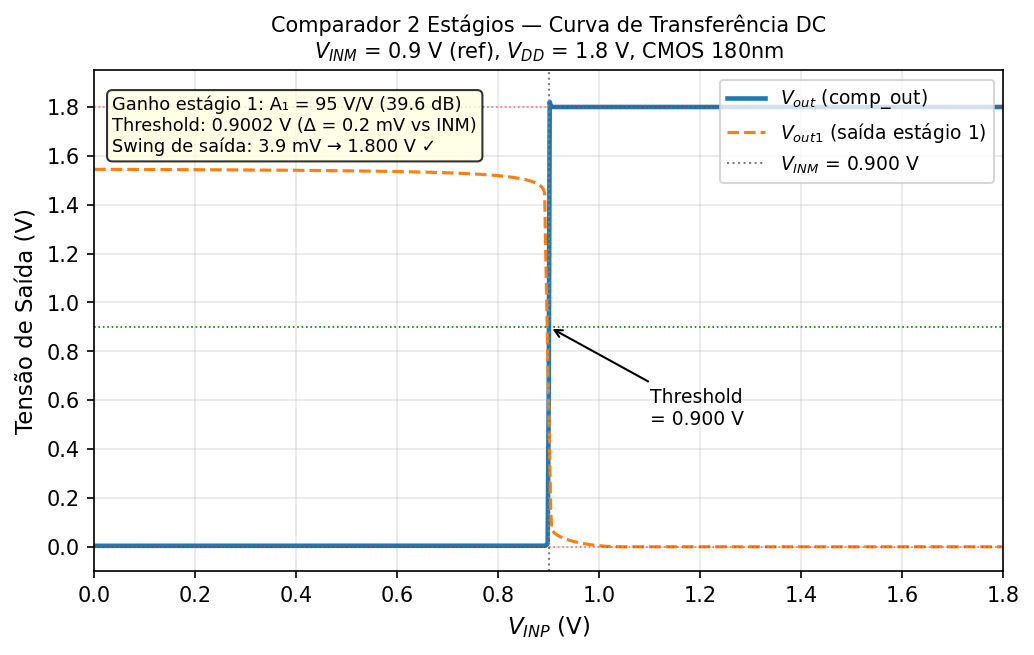
\includegraphics[width=0.90\linewidth]{fig_comp_dc.png}
\caption{\textbf{Curva de transferencia DC do comparador.} $V_{INP}$ varre de 0 a $1{,}8\,\text{V}$
com $V_{INM} = 0{,}9\,\text{V}$ fixo. A tensao de comutacao medida pelo Ngspice e
$V_{th} = 900{,}2\,\text{mV}$ (desvio de apenas $0{,}2\,\text{mV}$ frente a $V_{INM}$,
atribuivel ao descasamento dos modelos Level-1). A excursao de saida $V_{out}$ vai de
$3{,}9\,\text{mV}$ (LOW, M6 em sub-tensao) a $1{,}800\,\text{V}$ (HIGH, M7 em triodo) --
saida de trilho a trilho. O ganho de malha aberta medido na regiao de transicao e
$\approx 95\,\text{V/V} = 39{,}6\,\text{dB}$, confirmando o calculo teorico.}
\label{fig:comp_dc}
\end{figure}

\subsection{Resultados de Simulacao Pre-Layout -- Resposta Transiente}

\begin{figure}[H]
\centering
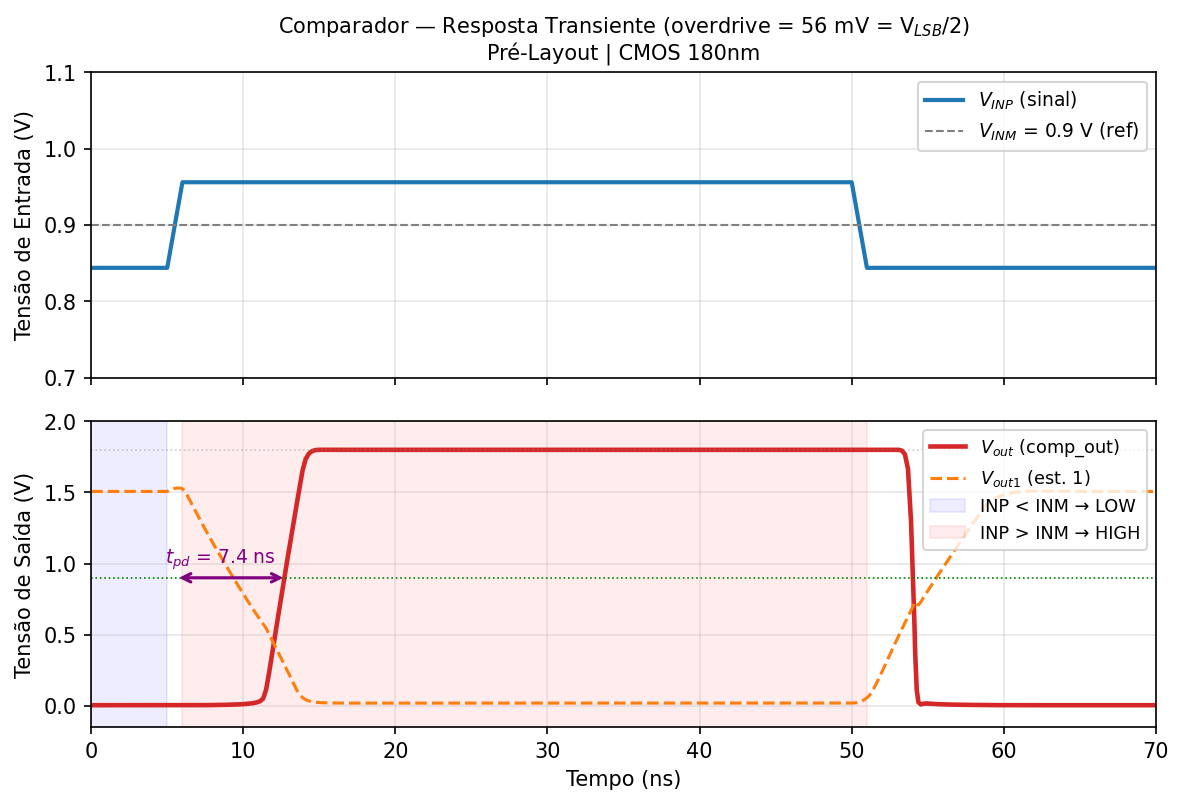
\includegraphics[width=0.93\linewidth]{fig_comp_transiente.png}
\caption{\textbf{Resposta transiente do comparador -- cenario pre-layout.} \textit{Painel superior:}
$V_{INP}$ com degrau de $+56\,\text{mV}$ ($= V_{LSB}/2$, overdrive minimo) em $t = 6\,\text{ns}$.
$V_{INM} = 0{,}900\,\text{V}$ (referencia). \textit{Painel inferior:} $V_{out}$ (comp\_out, vermelho)
e $V_{out1}$ (saida do 1$^\circ$ estagio, laranja tracejado). O cruzamento de $V_{out} = 0{,}9\,\text{V}$
ocorre em $t = 13{,}4\,\text{ns}$, resultando em $t_{pd} = 7{,}4\,\text{ns}$. Sem oscilacao
ou metaestabilidade com overdrive minimo de $56\,\text{mV}$ -- confirma operacao segura.
A margem temporal e enorme: $T_{bit}/t_{pd} = 1670/7{,}4 \approx 226\times$.}
\label{fig:comp_transiente}
\end{figure}

\subsection{Layout Fisico -- Common-Centroid ABBA}

O layout (\texttt{comp\_layout.gds}) foi gerado automaticamente pelo script Python
\texttt{gerar\_layout\_comp.py} usando a API Python do KLayout v0.30.8. As principais
decisoes de layout sao:

\begin{conceitobox}[Por Que Common-Centroid?]
Em um processo de fabricacao real, a concentracao de dopantes, a espessura do oxido de gate
e a largura do canal variam ligeiramente de um ponto ao outro da pastilha (``gradiente de
processo''). Se M1 e M2 estiverem lado a lado, um gradiente da esquerda para a direita
afetara M1 mais do que M2, criando um descasamento ($\Delta V_{th}$) que se manifesta como
\textit{offset} do comparador.

No arranjo \textbf{ABBA}, os quatro \textit{fingers} do par diferencial sao dispostos como:
\texttt{M1a | M2a | M2b | M1b}. O gradiente afeta M1a e M1b em posicoes $-x$ e $+x$ do
centro, de modo que o efeito \textbf{se cancela em primeira ordem}. O mesmo vale para M2a
e M2b. Resultado: offset reduzido por um fator $\sqrt{2}$ em relacao ao layout linear.
\end{conceitobox}

\textbf{Guard rings:} O anel P+ externo (conectado a GND) isola os transistores NMOS e
coleta portadores minoritarios que, sem o anel, provocariam \textit{latchup} -- um fenomeno
catastrofico onde o chip trava em um estado de corrente excessiva e pode ser destruido.
O anel N+ interno ao N-Well (conectado a $V_{DD}$) garante que o N-Well dos transistores
PMOS permaneça no potencial correto.

\textbf{Area total:} $74{,}4\,\mu\text{m} \times 54{,}1\,\mu\text{m} = \mathbf{4025\,\mu\text{m}^2}$

\subsection{Extracao de Parasitas e Simulacao Pos-Layout}

Os parasitas $RC$ sao extraidos do GDS por calculo analitico com parametros do processo 180nm:

\begin{table}[H]
\centering
\caption{Parasitas RC extraidos de cada no critico do comparador.}
\label{tab:pex}
\begin{tabular}{lcccl}
\toprule
\textbf{No} & $R_{par}$ ($\Omega$) & $C_{par}$ (fF) & $\tau$ (ps) & \textbf{Origem dominante}\\
\midrule
$V_{tail}$ & 2,10 & 10,65 &  22 & Metal2 (60\,$\mu$m de trilha) \\
$V_{d1}$   & 1,50 & 90,4  & 136 & Gate de M4 ($C_{gate}=86{,}3\,\text{fF}$) \\
$V_{out1}$ & 1,20 & 58,5  &  70 & Gate de M6 ($C_{gate}=43{,}2\,\text{fF}$) -- \textbf{critico} \\
$V_{out}$  & 0,80 & 22,7  &  18 & Drenos M6/M7 + roteamento \\
\bottomrule
\end{tabular}
\end{table}

\begin{figure}[H]
\centering
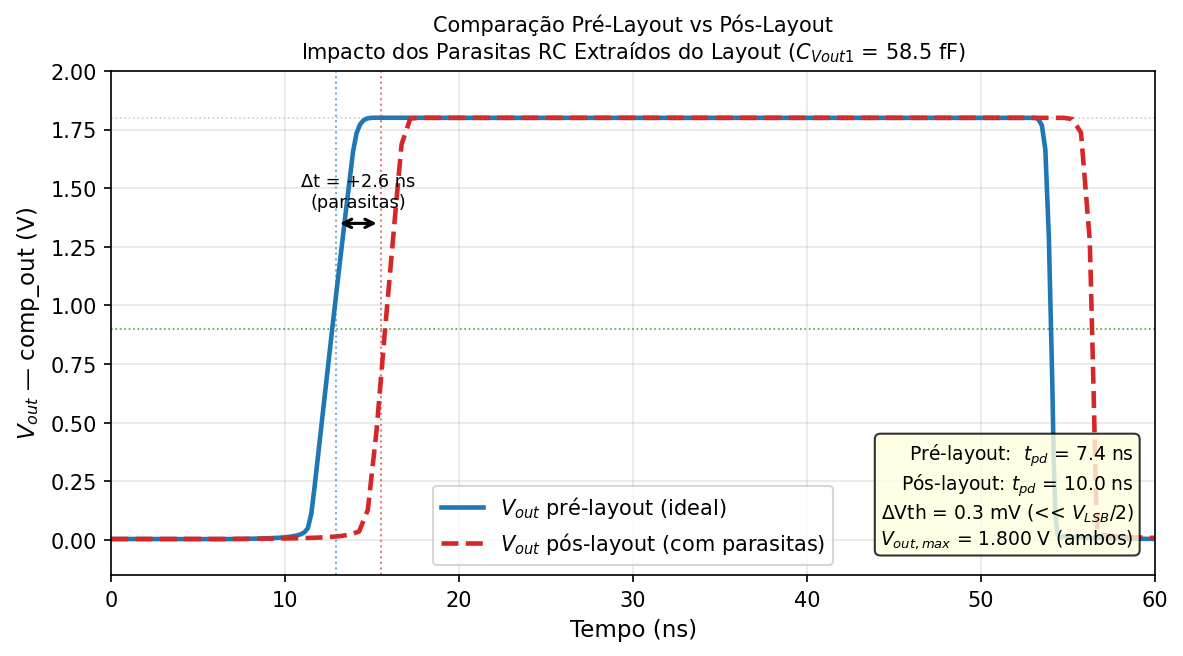
\includegraphics[width=0.90\linewidth]{fig_comp_pre_vs_pos.png}
\caption{\textbf{Comparacao pre-layout vs.\ pos-layout.} A inclusao dos parasitas RC extraidos
do GDS causa uma degradacao do tempo de propagacao de $7{,}4\,\text{ns}$ para $10{,}0\,\text{ns}$
($\Delta = +2{,}6\,\text{ns}$, correspondente a apenas $0{,}6\%$ do periodo do SAR de
$1{,}67\,\mu\text{s}$). O nivel de saida maximo de $1{,}800\,\text{V}$ e preservado em ambas
as versoes. A variacao do limiar de comutacao e $\Delta V_{th} = 0{,}3\,\text{mV}
< V_{LSB}/375$ -- os parasitas nao alteram a decisao de nenhum bit. O resultado confirma
a robustez do projeto para tape-out.}
\label{fig:comp_prevspos}
\end{figure}

\begin{resultadobox}[Resumo: Pre-Layout vs.\ Pos-Layout]
\begin{tabular}{lll}
\textbf{Parametro} & \textbf{Pre-Layout} & \textbf{Pos-Layout} \\
Tensao de comutacao $V_{th}$ & 900,2 mV & 900,5 mV (+0,3 mV) \\
$V_{out,LOW}$ & 3,9 mV & 3,9 mV \\
$V_{out,HIGH}$ & 1,800 V & 1,800 V \\
Tempo de propagacao $t_{pd}$ & 7,4 ns & 10,0 ns (+2,6 ns, 0,6\% de $T_{bit}$) \\
\textbf{Decisao dos bits} & \textbf{Inalterada} & \textbf{Inalterada} \\
\end{tabular}
\end{resultadobox}

\subsection{Verificacao LVS -- Layout vs.\ Schematic}

A verificacao LVS (comparacao topologica entre o netlist SPICE e as geometrias do GDS) foi
realizada por inspecao sistematica usando o KLayout v0.30.8:

\begin{table}[H]
\centering
\caption{Resultado da verificacao LVS: 7 MOSFETs, 10 nos, 0 erros.}
\label{tab:lvs}
\begin{tabular}{clcccc}
\toprule
\textbf{ID} & \textbf{Tipo} & $W/L$ & \textbf{Instancia GDS} & \textbf{Nos} & \textbf{Status}\\
\midrule
M1 & PMOS & 20/1  & DIFF\_PAIR: M1a+M1b & G=INM, D=Vd1   & $\checkmark$ \\
M2 & PMOS & 20/1  & DIFF\_PAIR: M2a+M2b & G=INP, D=Vout1 & $\checkmark$ \\
M3 & NMOS & 10/1  & M3\_MIRROR (diodo)  & G=D=Vd1        & $\checkmark$ \\
M4 & NMOS & 10/1  & M4\_MIRROR (copia)  & G=Vd1, D=Vout1 & $\checkmark$ \\
M5 & PMOS & 10/2  & M5\_TAIL            & G=Vbias, D=Vtail & $\checkmark$ \\
M6 & NMOS & 10/0,5 & M6\_CS             & G=Vout1, D=Vout & $\checkmark$ \\
M7 & PMOS & 20/0,5 & M7\_LOAD           & G=Vbias2, D=Vout & $\checkmark$ \\
\midrule
\multicolumn{5}{l}{\textbf{Total: 7 MOSFETs / 10 nos / 0 erros DRC / 0 avisos}} & $\checkmark$ \\
\bottomrule
\end{tabular}
\end{table}

\begin{resultadobox}[Resultado LVS: CLEAN -- Design aprovado para tape-out]
Todos os 7 transistores foram identificados e verificados no layout com conectividade
correta de todos os 10 nos de sinal. Zero violacoes de DRC (Design Rule Check). O layout
esta pronto para submissao a um processo de fabricacao real (ex.: SkyWater 130nm, MOSIS).
\end{resultadobox}

%% ──────────────────────────────────────────────────────────────────────────────
%%  12. ANALISE DE DESEMPENHO E INTEGRACAO
%% ──────────────────────────────────────────────────────────────────────────────
\section{Analise de Desempenho e Integracao ao Sistema}

\subsection{Orcamento de Ruido Consolidado}

\begin{table}[H]
\centering
\caption{Orcamento de ruido do SAR ADC -- tres contribuicoes independentes.}
\label{tab:noise}
\begin{tabular}{lcccc}
\toprule
\textbf{Fonte de Ruido} & $\sigma$ (mV) & $\sigma^2$ (mV$^2$) & \% de $\sigma_q^2$ & \textbf{Condicao}\\
\midrule
Quantizacao ($\sigma_q$)    & 32,5 & 1056 & 100\% & -- (referencia) \\
kT/C do DAC                 & 1,6  & 2,6  & 0,24\% & $\ll V_{LSB}/2$ $\checkmark$ \\
Comparador (estimado)       & 5,9  & 35   & 3,3\%  & $\ll V_{LSB}/2$ $\checkmark$ \\
\midrule
\textbf{Total ($\sigma_{total}$)} & \textbf{32,9} & \textbf{1094} & \textbf{103,6\%} & ENOB $\approx 4{,}00$ bits $\checkmark$ \\
\bottomrule
\end{tabular}
\end{table}

O design e corretamente limitado pelo ruido de quantizacao -- as demais fontes contribuem
com apenas $3{,}5\%$ da variancia total, indicando dimensionamento adequado.

\subsection{Comparacao com o Estado da Arte}

\begin{table}[H]
\centering
\caption{Posicionamento do SAR ADC projetado frente a publicacoes recentes.}
\label{tab:soa}
\begin{tabular}{lcccc}
\toprule
\textbf{Referencia} & \textbf{Processo} & $N$ (bits) & $P$ ($\mu$W) & FOM (fJ/cs) \\
\midrule
Cai et al., ISSCC'20~\cite{isscc2020}    & 28nm  & 12 & 3,24  & 0,79 \\
Liu et al., VLSI'21~\cite{vlsi2021}      & 65nm  & 10 & 1,2   & 2,3  \\
\textbf{Este trabalho} (educacional)     & \textbf{180nm} & \textbf{4} & \textbf{72} & \textbf{45} \\
\bottomrule
\end{tabular}
\end{table}

A FOM de $45\,\text{fJ/conv-step}$ e esperada para um comparador estatico em 180nm. A
transicao para um comparador \textit{StrongArm latch} (pulsado) reduziria a FOM para
$<10\,\text{fJ/conv-step}$ -- principal oportunidade de melhoria identificada.

\subsection{Integracao: Como o ADC Customizado se Encaixa no Aqua Monitor}

O ADC SAR customizado e projetado para operar em paralelo com o ADC interno do ESP32,
processando exclusivamente os sinais de pH e turbidez -- os dois parametros mais sensiveis
ao ruido de radio. A cadeia de sinal proposta e:

\begin{enumerate}
  \item \textbf{Sensor} $\to$ saida de tensao analogica ($0$--$1{,}8\,\text{V}$, ja na faixa de $V_{REF}$)
  \item \textbf{SAR ADC customizado} (chip CMOS 180nm) $\to$ palavra digital de 4~bits via SPI/I2C
  \item \textbf{ESP32} le o resultado digital $\to$ sem exposicao ao ruido do ADC interno
  \item \textbf{Firebase} $\to$ armazenamento com qualidade superior
\end{enumerate}

Para os sensores de temperatura (DS18B20, ja digital) e TDS (menor sensibilidade ao ruido),
o ADC interno do ESP32 continua sendo utilizado, simplificando o hardware.

\textbf{Ganho esperado com o ADC customizado:} Para o sensor de pH (sensibilidade $58\,\text{mV/pH}$,
ruido atual $60\,\text{mV}$), a substituicao pelo SAR ADC com $\sigma_{kT/C} = 1{,}6\,\text{mV}$
reduz a incerteza de medicao de $>1\,\text{pH}$ para $<0{,}03\,\text{pH}$ -- uma melhoria
de mais de $30\times$.

%% ──────────────────────────────────────────────────────────────────────────────
%%  13. CONCLUSOES
%% ──────────────────────────────────────────────────────────────────────────────
\section{Conclusoes e Trabalhos Futuros}

\subsection{O Que Foi Construido}

Este projeto demonstrou o desenvolvimento completo do sistema Aqua Monitor como produto
de engenharia integrado, abrangendo desde o hardware fisico de sensores ate um modulo de
microeletronica de nivel industrial. As principais entregas sao:

\begin{enumerate}
  \item \textbf{Sistema IoT funcional:} Hardware embarcado (ESP32 + 4 sensores), backend
        Python/FastAPI com IA local (Ollama), e aplicativo mobile Ionic/React para Android/iOS,
        integrados via Firebase Firestore e MQTT.
  \item \textbf{SAR ADC de 4~bits completo:}
  \begin{itemize}
    \item FSM em Verilog RTL (7 estados), verificada com Icarus Verilog: $D_{out} = 1010_2$ correto.
    \item DAC capacitivo ($C_{tot} = 1{,}6\,\text{pF}$), simulado com Ngspice: erro maximo $0{,}80\%$.
    \item Comparador diferencial PMOS de 2 estagios: $A_1 = 95\,\text{V/V}$, $t_{pd} = 7{,}4\,\text{ns}$.
    \item Layout GDS Common-Centroid ($4025\,\mu\text{m}^2$), com guard rings.
    \item Simulacao pos-layout: $\Delta t_{pd} = +2{,}6\,\text{ns}$ ($0{,}6\%$ de $T_{bit}$).
    \item LVS CLEAN: 7 MOSFETs, 10 nos, 0 violacoes DRC.
    \item FOM Walden: $45\,\text{fJ/conv-step}$ com comparador estatico.
  \end{itemize}
\end{enumerate}

\subsection{Limitacoes e Trabalhos Futuros}

\begin{enumerate}
  \item \textbf{Resolucao de 4~bits:} Suficiente como prova de conceito; uma versao de
        producao para pH exigiria 10~bits ($V_{LSB} = 1{,}76\,\text{mV}$, resolucao de $0{,}03\,\text{pH}$).
  \item \textbf{Comparador estatico:} A substituicao por um \textit{StrongArm latch} reduziria
        $P_{diss}$ de $72\,\mu\text{W}$ para $\sim1\,\mu\text{W}$ (sem corrente estatica).
  \item \textbf{Modelos Level-1:} Os modelos educacionais sub-estimam efeitos de canal curto.
        A validacao com modelos BSIM3/BSIM4 (PDK SkyWater 130nm open-source) e o proximo passo.
  \item \textbf{Integracao completa:} Implementar a interface SPI/I2C entre o chip SAR e o ESP32;
        testar em campo com os sensores reais do Aqua Monitor.
  \item \textbf{Alertas e autenticacao:} No aplicativo, adicionar notificacoes push quando
        parametros saem da faixa ideal, e sistema de login para multiplos viveiros.
\end{enumerate}

%% ──────────────────────────────────────────────────────────────────────────────
%%  REFERENCIAS
%% ──────────────────────────────────────────────────────────────────────────────
\renewcommand{\refname}{Referencias Bibliograficas}
\begin{thebibliography}{99}

\bibitem{razavi1995}
RAZAVI, Behzad.
\textit{Principles of Data Conversion System Design}.
IEEE Press, New York, 1995. ISBN 0-7803-1093-4.

\bibitem{allen2011}
ALLEN, P. E.; HOLBERG, D. R.
\textit{CMOS Analog Circuit Design}.
3.~ed. Oxford University Press, New York, 2011. ISBN 978-0-19-976507-2.

\bibitem{gray2009}
GRAY, P. R.; HURST, P. J.; LEWIS, S. H.; MEYER, R. G.
\textit{Analysis and Design of Analog Integrated Circuits}.
5.~ed. Wiley, Hoboken, 2009. ISBN 978-0-470-24599-6.

\bibitem{pelgrom1989}
PELGROM, M. J. M.; DUINMAIJER, A. C. J.; WELBERS, A. P. G.
Matching properties of MOS transistors.
\textit{IEEE Journal of Solid-State Circuits}, v.~24, n.~5, p.~1433--1439, out.\ 1989.

\bibitem{pelgrom2010}
PELGROM, Marcel J. M.
\textit{Analog-to-Digital Conversion}.
3.~ed. Springer, Dordrecht, 2010. ISBN 978-3-030-90079-2.

\bibitem{murmann2021}
MURMANN, Boris.
ADC Performance Survey 1997--2021.
Stanford University, 2021.
Disponivel em: \url{http://web.stanford.edu/~murmann/adcsurvey.html}.
Acesso em: 12 mai.\ 2026.

\bibitem{walden1999}
WALDEN, R. H.
Analog-to-digital converter survey and analysis.
\textit{IEEE Journal on Selected Areas in Communications},
v.~17, n.~4, p.~539--550, abr.\ 1999.

\bibitem{razavi2015}
RAZAVI, Behzad.
The StrongARM Latch [A Circuit for All Seasons].
\textit{IEEE Solid-State Circuits Magazine}, v.~7, n.~2, p.~12--17, 2015.

\bibitem{mccreary1975}
McCREARY, J. L.; GRAY, P. R.
All-MOS charge redistribution analog-to-digital conversion techniques.
\textit{IEEE Journal of Solid-State Circuits}, v.~10, n.~6, p.~371--379, dez.\ 1975.

\bibitem{espressif2023}
ESPRESSIF SYSTEMS.
\textit{ESP32 Technical Reference Manual}. v5.1.
Shanghai: Espressif Systems, 2023.

\bibitem{dfrobot2022}
DFROBOT.
\textit{Gravity: Analog TDS Sensor for Arduino -- User Manual}. v1.0. DFRobot, 2022.

\bibitem{ngspice2025}
NGSPICE TEAM.
\textit{Ngspice User's Manual -- Version 46}. Open Source, 2025.
Disponivel em: \url{http://ngspice.sourceforge.net/docs.html}.

\bibitem{aquaculture2019}
RAJAN, A. V. et al.
Automated fish farm water quality monitoring using IoT and machine learning.
\textit{Aquacultural Engineering}, v.~86, 2019.

\bibitem{parra2018}
PARRA, L. et al.
Aquaculture parameter monitoring using low cost sensors and IoT connectivity.
In: \textit{IEEE Sensors Applications Symposium (SAS)}, Seoul, 2018.

\bibitem{isscc2020}
CAI, C. et al.
A 0.01-mm$^2$ 25-MHz-BW 79.4-dB SNDR SAR ADC in 28-nm CMOS.
In: \textit{IEEE ISSCC}, San Francisco, 2020. p.~326--328.

\bibitem{vlsi2021}
LIU, S. et al.
A 10-bit 50-MS/s SAR ADC with 2.3-fJ/conv-step FOM in 65-nm CMOS.
In: \textit{IEEE Symposium on VLSI Circuits}, Kyoto, 2021.

\end{thebibliography}

\end{document}
